\section{Introdução}
Este documento detalha a modelagem lógica e física do banco de dados,
especificando tabelas, tipos de dados, chaves e os relacionamentos que sustentam
a lógica de negócio do sistema de gerenciamento de projetos. Ao fim do documento,
o diagrama UML e o script SQL gerado nessa etapa são revelados.
\section{Diagrama do Banco de Dados}

\begin{figure}[H]
    \centering
    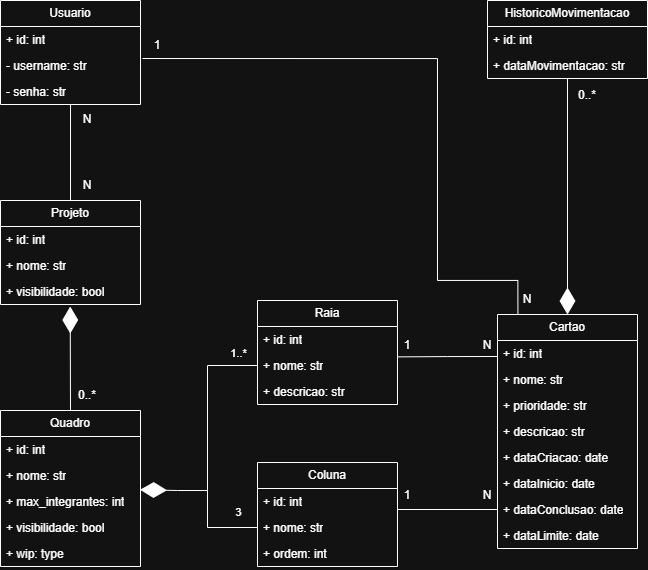
\includegraphics[width=0.8\textwidth]{./images/DiagramaBD.jpeg}
    \caption{Diagrama Físico do Banco de Dados.}
\end{figure}

\section{Dicionário de Dados}
Esta seção detalha a modelagem lógica do banco de dados. 
Onde são especificadas as tabelas, seus atributos e detalhes de relacionamento.

\subsection{Tabela: usuarios}
\textbf{Propósito:} Armazena as informações de autenticação e identificação dos usuários do sistema.

\begin{table}[H]
    \centering
    \begin{tabular}{|l|l|p{8cm}|}
        \hline
        \textbf{Coluna} & \textbf{Tipo de Dado} & \textbf{Restrições / Chaves} \\
        \hline
        id & BIGINT & PK \\
        \hline
        username & VARCHAR & \\
        \hline
        senha & VARCHAR & \\
        \hline
    \end{tabular}
    \caption{Estrutura da tabela usuarios.}
\end{table}
\noindent \textbf{Relacionamentos:} Associação 1:N com \texttt{cartoes} (como responsável); Associação N:N com \texttt{projetos}.

\subsection{Tabela: projetos}
\textbf{Propósito:} Define os projetos que contêm quadros e gerencia o acesso dos usuários.

\begin{table}[H]
    \centering
    \begin{tabular}{|l|l|p{8cm}|}
        \hline
        \textbf{Coluna} & \textbf{Tipo de Dado} & \textbf{Restrições / Chaves} \\
        \hline
        id & BIGINT & PK \\
        \hline
        nome & VARCHAR & \\
        \hline
        visibilidade & ENUM & \\
        \hline
    \end{tabular}
    \caption{Estrutura da tabela projetos.}
\end{table}
\noindent \textbf{Relacionamentos:} Associação N:N com \texttt{usuarios} (intermediado pela tabela \texttt{usuarios\_projetos}); Composição 0..* com \texttt{quadros}.

\subsection{Tabela: usuarios\_projetos}
\textbf{Propósito:} Gerencia a permissão de acesso de usuários aos projetos. Atua como tabela associativa (junction table).

\begin{table}[H]
    \centering
    \begin{tabular}{|l|l|p{8cm}|}
        \hline
        \textbf{Coluna} & \textbf{Tipo de Dado} & \textbf{Restrições / Chaves} \\
        \hline
        usuario\_id & BIGINT & PK, FK referenciando usuarios(id) \\
        \hline
        projeto\_id & BIGINT & PK, FK referenciando projetos(id) \\
        \hline
    \end{tabular}
    \caption{Estrutura da tabela usuarios\_projetos.}
\end{table}
\noindent \textbf{Relacionamentos:} Resolve o relacionamento N:N entre as entidades Usuários e Projetos.

\subsection{Tabela: quadros}
\textbf{Propósito:} Representa o ambiente de trabalho (quadro) que agrupa colunas e raias dentro de um projeto específico.

\begin{table}[H]
    \centering
    \begin{tabular}{|l|l|p{8cm}|}
        \hline
        \textbf{Coluna} & \textbf{Tipo de Dado} & \textbf{Restrições / Chaves} \\
        \hline
        id & BIGINT & PK \\
        \hline
        nome & VARCHAR & \\
        \hline
        max\_integrantes & INT & \\
        \hline
        visibilidade & ENUM & \\
        \hline
        wip & INT & \\
        \hline
        projeto\_id & BIGINT & FK referenciando projetos(id) \\
        \hline
    \end{tabular}
    \caption{Estrutura da tabela quadros.}
\end{table}
\noindent \textbf{Relacionamentos:} Associação N:N com \texttt{usuarios}; Composição 1:3 com \texttt{colunas}, 1:N com \texttt{raias}.

\subsection{Tabela: colunas}
\textbf{Propósito:} Define as etapas do fluxo de trabalho (ex: A Fazer, Fazendo, Feito) dentro de um quadro.

\begin{table}[H]
    \centering
    \begin{tabular}{|l|l|p{8cm}|}
        \hline
        \textbf{Coluna} & \textbf{Tipo de Dado} & \textbf{Restrições / Chaves} \\
        \hline
        id & BIGINT & PK \\
        \hline
        nome & ENUM & \\
        \hline
        ordem & INT & \\
        \hline
        quadro\_id & BIGINT & FK referenciando quadros(id) \\
        \hline
    \end{tabular}
    \caption{Estrutura da tabela colunas.}
\end{table}
\noindent \textbf{Relacionamentos:} Associação 1:N com \texttt{cartoes}; Composição 1:3 com \texttt{quadro}.

\subsection{Tabela: raias}
\textbf{Propósito:} Permite categorizar ou segmentar os cartões horizontalmente (swimlanes) dentro de um quadro.

\begin{table}[H]
    \centering
    \begin{tabular}{|l|l|p{8cm}|}
        \hline
        \textbf{Coluna} & \textbf{Tipo de Dado} & \textbf{Restrições / Chaves} \\
        \hline
        id & BIGINT & PK \\
        \hline
        nome & VARCHAR & \\
        \hline
        descricao & TEXT & \\
        \hline
        quadro\_id & BIGINT & FK referenciando quadros(id) \\
        \hline
    \end{tabular}
    \caption{Estrutura da tabela raias.}
\end{table}
\noindent \textbf{Relacionamentos:} Associação 1:N com \texttt{cartoes}; Composição 1:N com \texttt{quadro}.

\subsection{Tabela: cartoes}
\textbf{Propósito:} Armazena as tarefas ou itens de trabalho, contendo detalhes de execução, prazos e rastreamento.

\begin{table}[H]
    \centering
    \begin{tabular}{|l|l|p{8cm}|}
        \hline
        \textbf{Coluna} & \textbf{Tipo de Dado} & \textbf{Restrições / Chaves} \\
        \hline
        id & BIGINT & PK \\
        \hline
        nome & VARCHAR & \\
        \hline
        descricao & TEXT & \\
        \hline
        prioridade & ENUM & \\
        \hline
        data\_criacao & DATETIME & \\
        \hline
        data\_inicio & DATETIME & \\
        \hline
        data\_conclusao & DATETIME & \\
        \hline
        data\_limite & DATE & \\
        \hline
        responsavel\_id & BIGINT & FK referenciando usuarios(id) \\
        \hline
        coluna\_id & BIGINT & FK referenciando colunas(id) \\
        \hline
        raia\_id & BIGINT & FK referenciando raias(id) \\
        \hline
    \end{tabular}
    \caption{Estrutura da tabela cartoes.}
\end{table}
\noindent \textbf{Relacionamentos:} Associação 1:N com \texttt{usuarios}; Composição 0:N com \texttt{historico\_movimentacoes}.

\subsection{Tabela: historico\_movimentacoes}
\textbf{Propósito:} Registra o histórico completo de movimentações de um cartão entre colunas e raias, permitindo auditoria de quem realizou a alteração e quando.

\begin{table}[H]
    \centering
    \begin{tabular}{|l|l|p{8cm}|}
        \hline
        \textbf{Coluna} & \textbf{Tipo de Dado} & \textbf{Restrições / Chaves} \\
        \hline
        id & BIGINT & PK \\
        \hline
        cartao\_id & BIGINT & FK referenciando cartoes(id) \\
        \hline
        coluna\_origem\_id & BIGINT & FK referenciando colunas(id) \\
        \hline
        coluna\_destino\_id & BIGINT & FK referenciando colunas(id) \\
        \hline
        raia\_origem\_id & BIGINT & FK referenciando raias(id) \\
        \hline
        raia\_destino\_id & BIGINT & FK referenciando raias(id) \\
        \hline
        usuario\_id & BIGINT & FK referenciando usuarios(id) \\
        \hline
        data\_movimentacao & DATETIME & \\
        \hline
    \end{tabular}
    \caption{Estrutura da tabela historico\_movimentacoes.}
\end{table}
\noindent \textbf{Relacionamentos:} Vinculado a um \texttt{cartao}, duas \texttt{colunas} (origem/destino), duas \texttt{raias} (origem/destino) e um \texttt{usuario} executor.
